%%%%%%%%%%%%%%%%%%%%%%%%%%%%%%%%%%%%%%%%%%%%%%%%%%%%%%%%%%%%%%%%%%%%%%%%%%%%%%
%
% Fourier Transform Pairs
%
%%%%%%%%%%%%%%%%%%%%%%%%%%%%%%%%%%%%%%%%%%%%%%%%%%%%%%%%%%%%%%%%%%%%%%%%%%%%%%

\chapter{Fourier Transform Pairs}

Throughout this chapter,

\[
f(x,y)\xleftrightarrow{\ \FT\ }F(\fx,\fy).
\]

%%%%%%%%%%%%%%%%%%%%%%%%%%%%%%%%%%%%%%%%%%%%%%%%%%%%%%%%%%%%%%%%%%%%%%%%%%%%%%
\section{Frequency Convention}

\begin{center}
\begin{tabular}{lll}
\toprule
Function $f(x,y)$ & Fourier Transform $F(\fx,\fy)$ & Notes\\
\midrule

$\displaystyle
1
$
&
$\displaystyle
\delta(\fx)\delta(\fy)
$
&
Constant

\\[0.5cm]

$\displaystyle
\delta(x)\delta(y)
$
&
$\displaystyle
1
$
&
Dirac delta

\\[0.5cm]

$\displaystyle
\rect\!\left(\frac{x}{a}\right)
\rect\!\left(\frac{y}{b}\right)
$
&
$\displaystyle
|ab|\,
\sinc(a\fx)\sinc(b\fy)
$
&
Rectangular aperture

\\[0.5cm]

$\displaystyle
\tri\left(\frac{x}{a}\right)\tri\left(\frac{x}{b}\right)
$
&
$\displaystyle
|ab|\sinc^2(a\fx)\sinc^2(b\fy)
$
&
Triangle

\\[0.5cm]

$\displaystyle
e^{-\pi(x^2/a^2+y^2/b^2)}
$
&
$\displaystyle
|ab|\,
e^{-\pi(a^2\fx^2+b^2\fy^2)}
$
&
Gaussian
\\[0.5cm]

$\displaystyle
\comb(ax)\comb(by)
$
&
$\displaystyle
\frac{1}{|ab|}\comb\left(\frac{\fx}{a}\right)\comb\left(\frac{\fy}{b}\right)
$
&
Dirac comb

\\[0.5cm]

$\displaystyle
e^{\iu 2\pi(f_{0x}x+f_{0y}y)}
$
&
$\displaystyle
\delta(\fx-f_{0x})
\delta(\fy-f_{0y})
$
&
Plane wave

\\[0.5cm]

$\displaystyle
\circf\left(\frac{r}{R}\right)
$
&
$\displaystyle
2\pi R^2\frac{J_1(2\pi R\rho)}{2 \pi R\rho}=\pi R^2\jinc(2R\rho)
$
&
Circular aperture

\\

\bottomrule
\end{tabular}
\end{center}

where

\[
r=\sqrt{x^2+y^2},
\qquad
\rho=\sqrt{\fx^2+\fy^2}.
\]

%%%%%%%%%%%%%%%%%%%%%%%%%%%%%%%%%%%%%%%%%%%%%%%%%%%%%%%%%%%%%%%%%%%%%%%%%%%%%%
\pagebreak
\section{Wave-Vector Convention}

Using

\[
\mathbf{k}=2\pi\mathbf{f},
\]

the corresponding transform pairs are

\begin{center}
\begin{tabular}{lll}
\toprule
Function $f(x,y)$ & Fourier Transform $F(\kx,\ky)$ & Notes\\
\midrule

$\displaystyle
1
$
&
$\displaystyle
(2\pi)^2\delta(\kx)\delta(\ky)
$
&
Constant

\\[0.5cm]

$\displaystyle
\delta(x)\delta(y)
$
&
$\displaystyle
1
$
&
Dirac delta

\\[0.5cm]

$\displaystyle
\rect\!\left(\frac{x}{a}\right)
\rect\!\left(\frac{y}{b}\right)
$
&
$\displaystyle
|ab|\,
\sinc\left(\frac{a\kx}{2\pi}\right)
\sinc\left(\frac{b\ky}{2\pi}\right)
$
&
Rectangular aperture

\\[0.5cm]

$\displaystyle
\tri\left(\frac{x}{a}\right)\tri\left(\frac{x}{b}\right)
$
&
$\displaystyle
|ab|\sinc^2\left(\frac{a\kx}{2\pi}\right)
\sinc^2\left(\frac{b\ky}{2\pi}\right)
$
&
Triangle

\\[0.5cm]

$\displaystyle
e^{-\pi(x^2/a^2+y^2/b^2)}
$
&
$\displaystyle
|ab|\,
e^{-\frac{1}{4\pi}(a^2\kx^2+b^2\ky^2)}
$
&
Gaussian
\\[0.5cm]

$\displaystyle
\comb(ax)\comb(by)
$
&
$\displaystyle
\frac{1}{|ab|}\comb\left(\frac{\kx}{2\pi a}\right)\comb\left(\frac{\ky}{2\pi b}\right)
$
&
Dirac comb

\\[0.5cm]
$\displaystyle
e^{\iu(k_{0x}x+k_{0y}y)}
$
&
$\displaystyle
(2\pi)^2
\delta(\kx-k_{0x})
\delta(\ky-k_{0y})
$
&
Plane wave

\\[0.5cm]

$\displaystyle
\circf\left(\frac{r}{R}\right)
$
&
$\displaystyle
2\pi R^2\frac{J_1(R k)}{R k}=\pi R^2\jinc\left(\frac{R k}{\pi}\right)
$
&
Circular aperture
\\

\bottomrule
\end{tabular}
\end{center}

where

\[
r=\sqrt{x^2+y^2},
\qquad
k=\sqrt{\kx^2+\ky^2}.
\]
\pagebreak
%\section{Plots}
\begin{figure}[b]
    \centering
    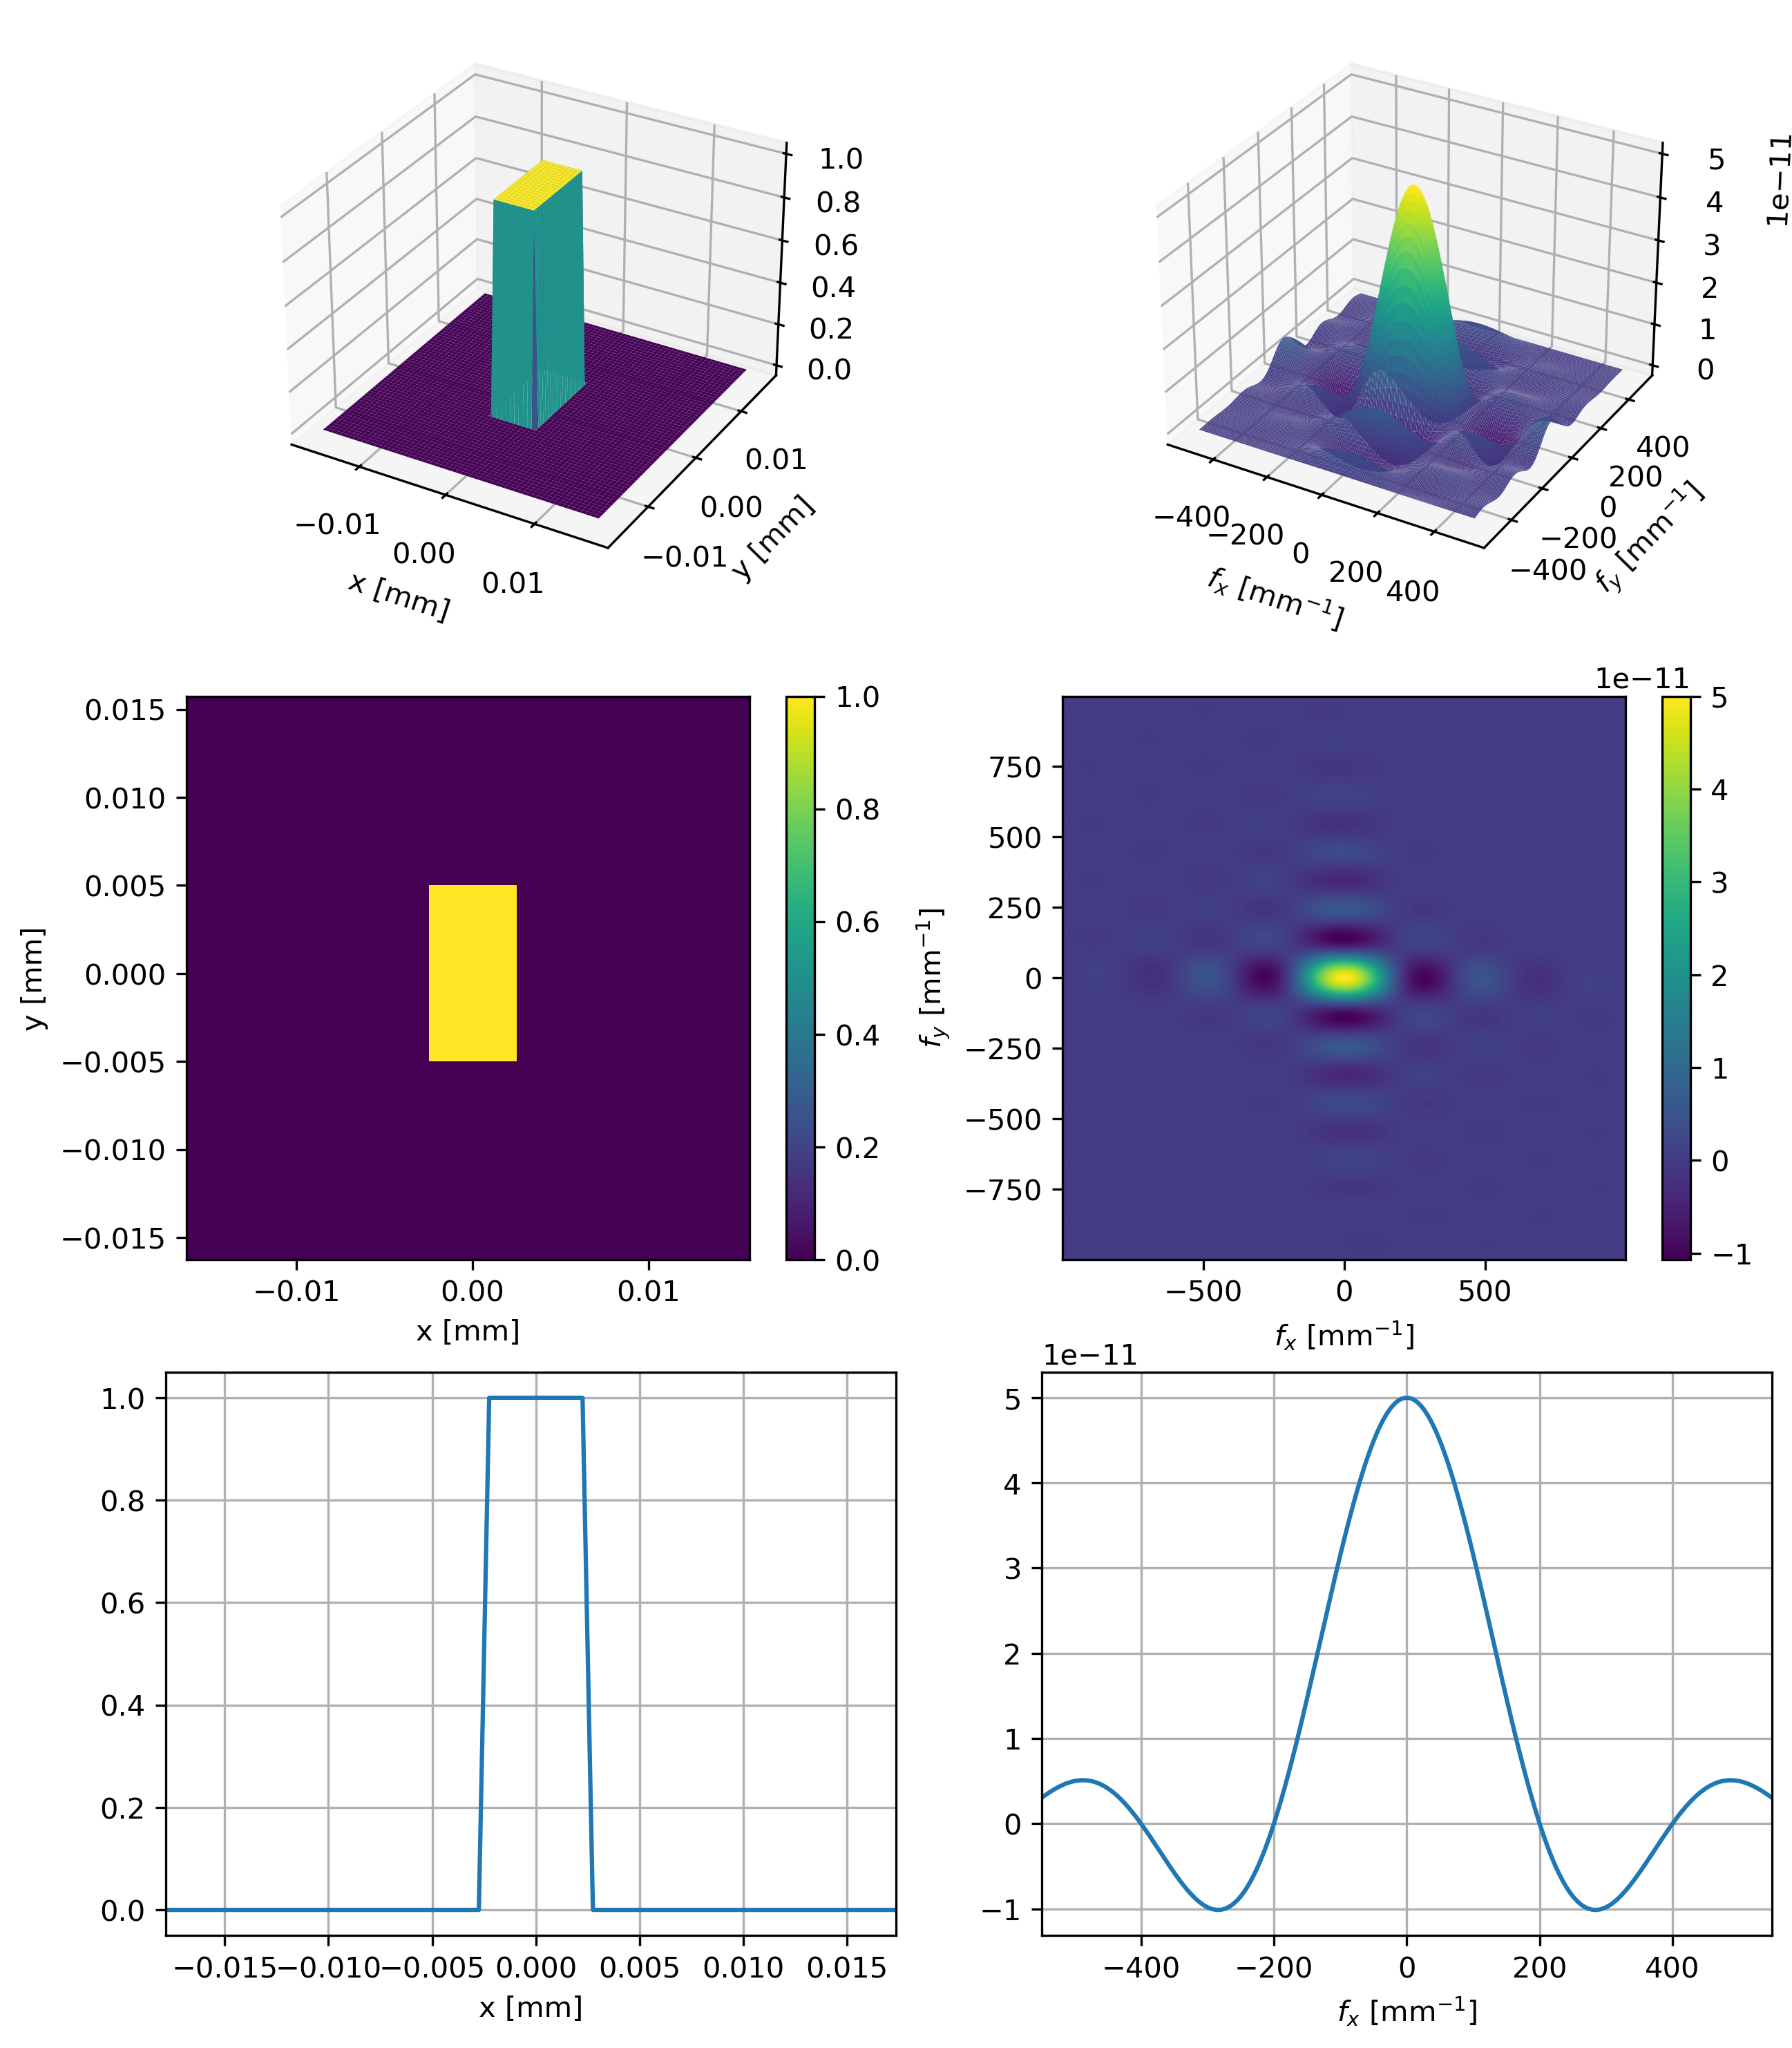
\includegraphics[width=1\linewidth]{docs/handbook/fig/rect_Fourier.png}
    \caption{Fourier Transform of a rectangle function with $a=5\mu$m and $b=10\mu$m. On the left column the rectangle, on the right column the Fourier transform.}
    \label{fig:rectFourier}
\end{figure}
\begin{figure}
    \centering
    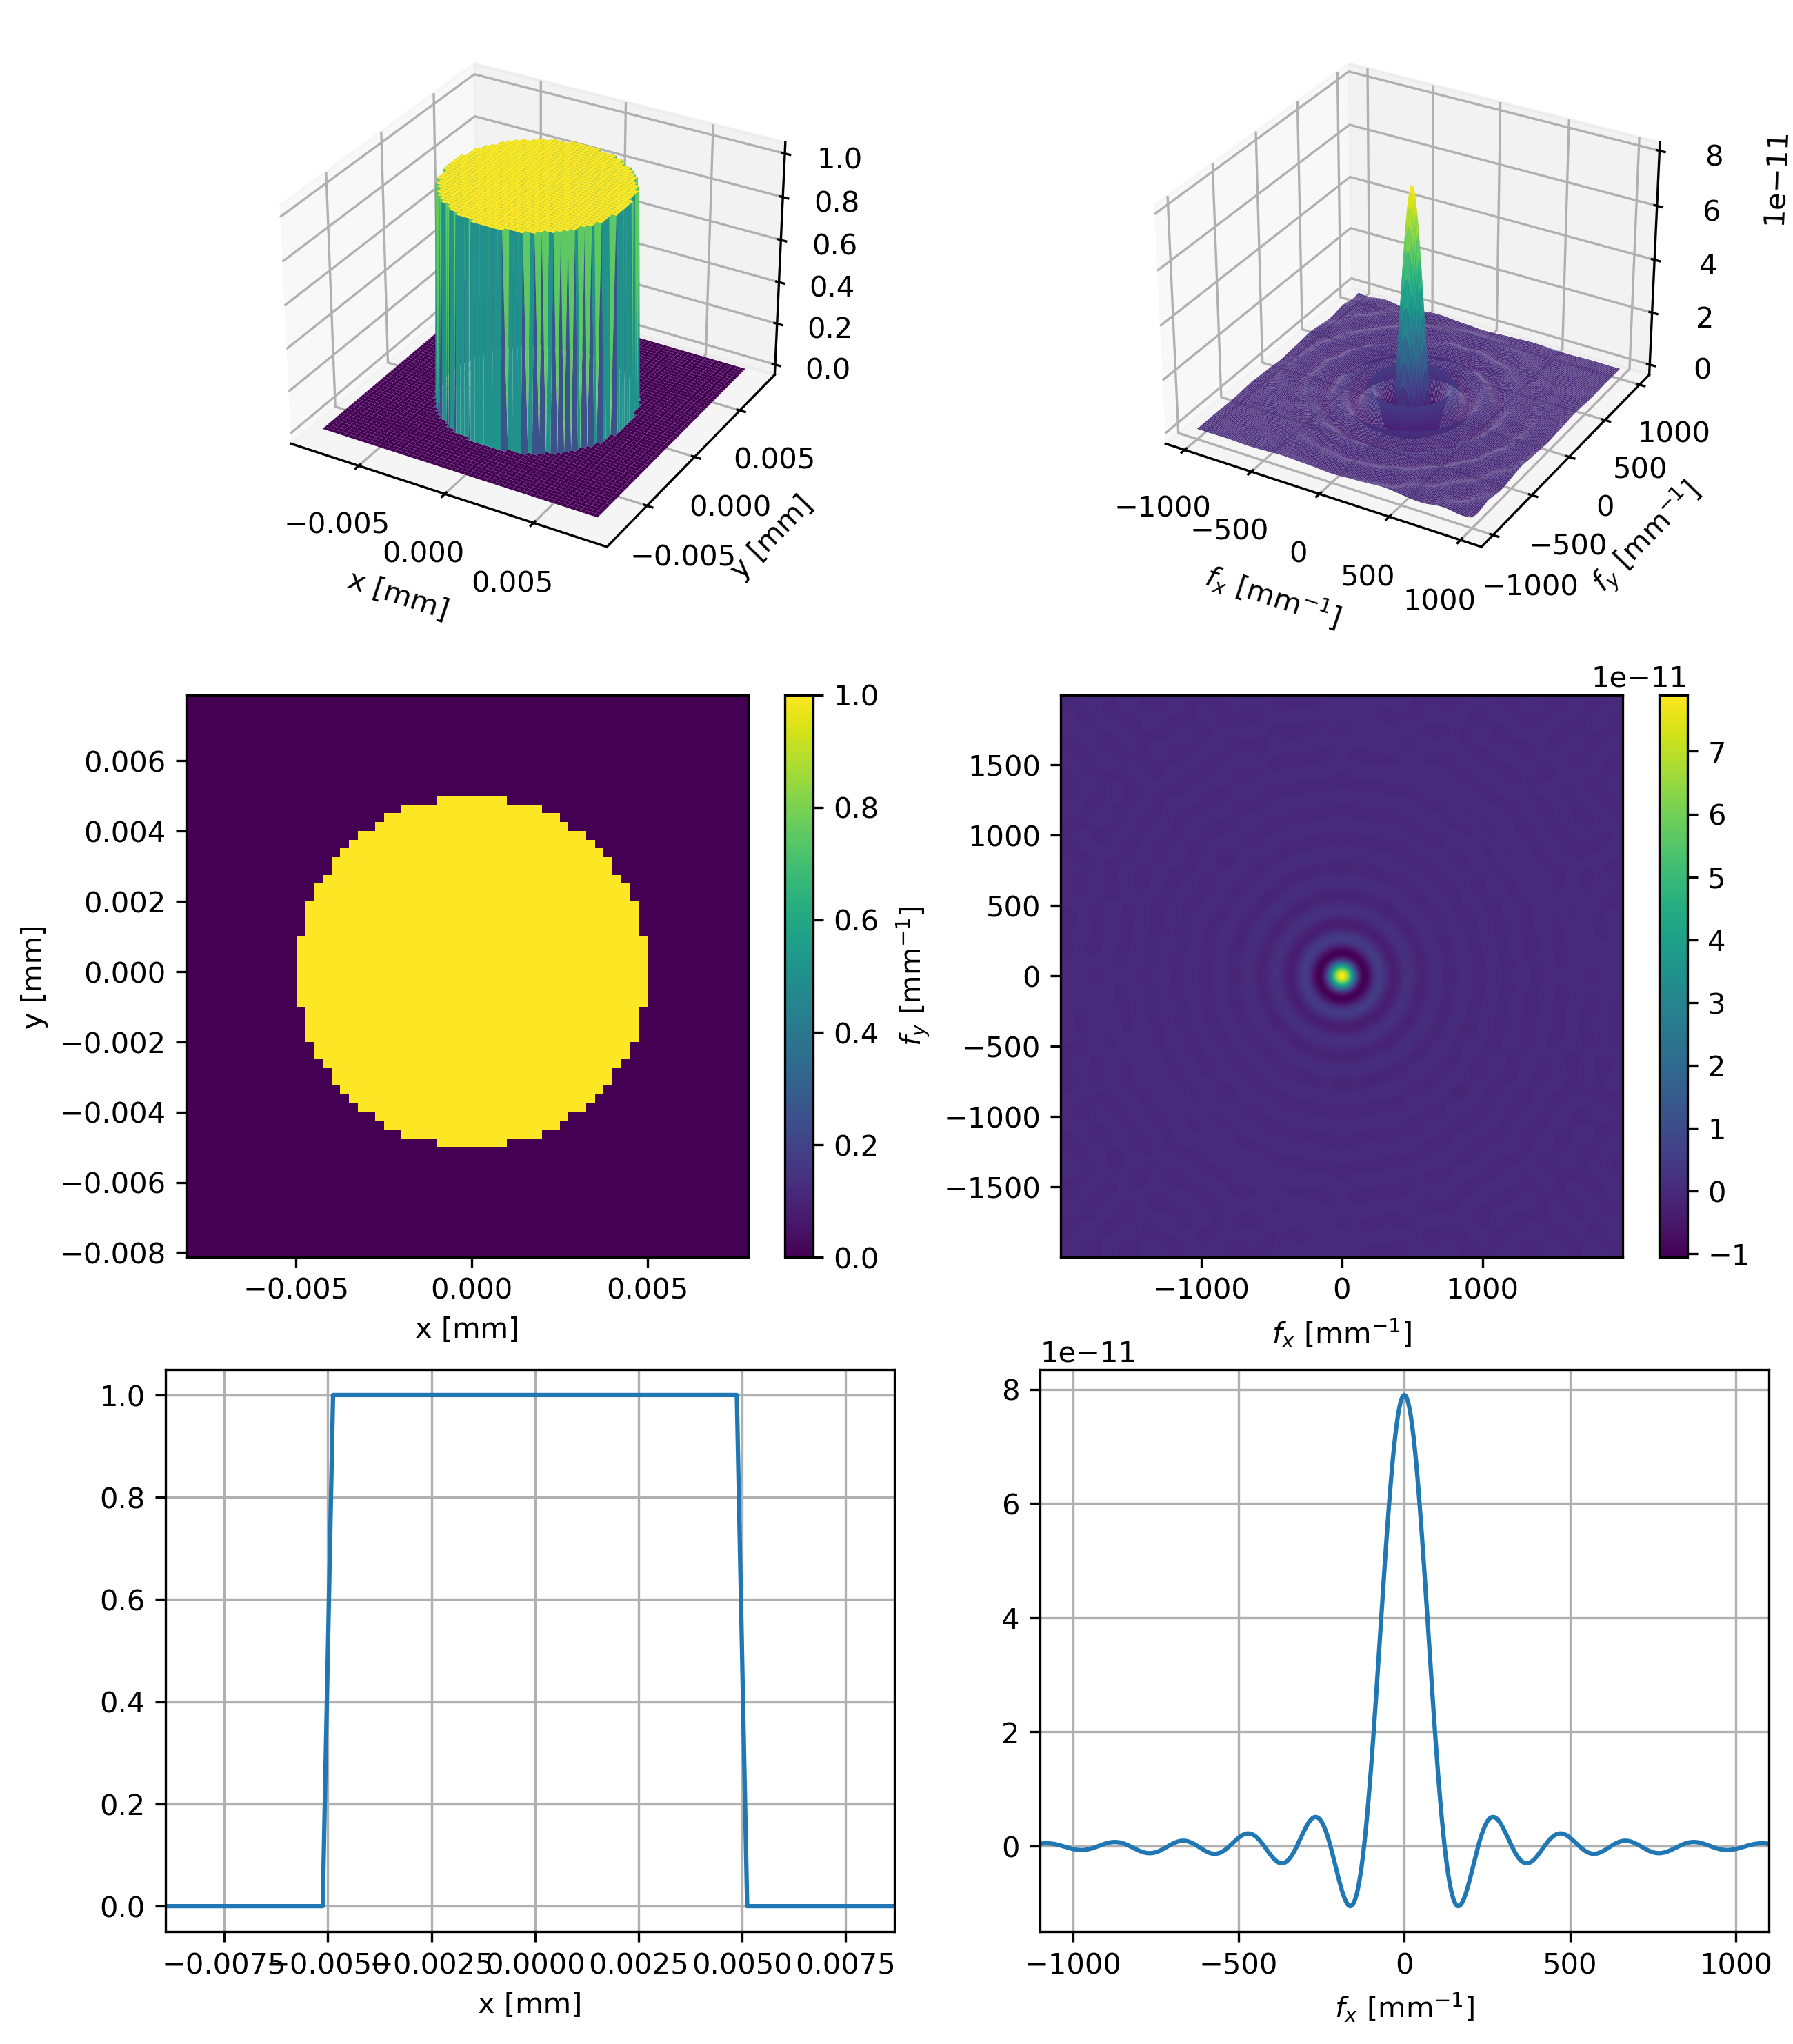
\includegraphics[width=1.0\linewidth]{docs/handbook/fig/circle_Fourier.png}
    \caption{Fourier Transform of a circle function with $R=5\mu$m. On the left column the circle, on the right column the Fourier transform.}
    \label{fig:rectFourier}
\end{figure}